\chapter{Methodology}
We consider a team of $N$ UAVs in an unknown environment, each of which has a range of sensing area detected by its sensor. By knowing the positions of obstacles and their teammates in the sensing area, every UAV should fly from the starting area to the goal point with the constraints of avoiding obstacles and keeping a safe distance among teammates. Besides, a compact formation needs to be figured during the whole mission in various testing environments.

\section{Model Formulation}

The starting point of each UAV and the common goal point are given by
\begin{equation}
\begin{aligned}
& Start_{i} = x_{i}(t_{start}),  y_{i}(t_{start}) \\
& End = x_{end},  y_{end}
\end{aligned}
\end{equation}
where $x_{i}(t_{start}), y_{i}(t_{start})$ is the position of $i$th UAV at the starting time $t_{start}$. We then use the linear discrete-time model ($t_{0}, t_{1}, ..., t_{n}$) for the kinematic equations
\begin{equation} 
\begin{aligned}
& x_{i}(t_{n}) = x_{i}(t_{0}) + \int_{t_{0}}^{t_{n}} v_{i}(t) \cdot cos\theta_{i}(t)dt \\
& y_{i}(t_{n}) = y_{i}(t_{0}) + \int_{t_{0}}^{t_{n}} v_{i}(t) \cdot sin\theta_{i}(t)dt \\
& \theta_{i}(t) = \theta_{i}(t_{0}) + \int_{t_{0}}^{t} \omega_{i}(\hat{t})dt
\end{aligned}
\end{equation}
for all $i\in$\{1, 2, ..., $N$\}, where $(x_{i}(t_{n})$, $y_{i}(t_{n}))$ is the position of $i$th UAV, $v_{i}(t)$ is the velocity, and $\theta_{i}(t)$ is the orientation at time $t$. $\theta(t)$ is determined by the angular velocity $\omega$ at time $\hat{t}\in[t_{0}, t_{n}]$. In other words, $v$ and $\omega$ are two inputs which control the motion of UAVs at any time. In practice, the vehicles have the following speed and angular velocity constraints: 
\begin{equation} 
\begin{aligned}
& 0\leq v_{i}(t)\leq v_{\max}\\
& -\omega_{\max}\leq\omega_{i}(t)\leq\omega_{\max}
\end{aligned}
\end{equation}

On a battlefield of high uncertainty, We use the dynamic windows approach for each UAV to predict $j$ trajectories $T^{j}_{i}$ in a time window [$t_{0}$, $t_{T}$]. Each of the trajectories consists a series of nodes from time $t_{0}$ to time $t_{T}$, thus we define the last node of $T^{j}_{i}$ at time $t_{T}$ as the predicted points $P^{j}_{i}$.

\begin{equation}
\begin{aligned}
& T^{j}_{i} = \{(x^{j}_{i}(t_{0}), y^{j}_{i}(t_{0})), (x^{j}_{i}(t_{1}), y^{j}_{i}(t_{1})),... P^{j}_{i} \} \\
& P^{j}_{i} = x^{j}_{i}(t_{T}), y^{j}_{i}(t_{T})
\end{aligned}
\end{equation}

The above predicted possible trajectories is depended on the inputs ${v}$ and ${\omega}$ controlled by time windows, and the range of ${v}$ and ${\omega}$ can be adjusted more tightly from equation 3.3 as follows:

\begin{equation}
\begin{aligned}
& \max(0, \hat v-a\cdot \hat{t})\leq v\leq \min(v_{max}, \hat v+a\cdot\hat{t})\\
& \max(0, \hat \omega-\Delta \omega\cdot \hat{t})\leq \omega\leq \min(v_{max}, \hat \omega+\Delta \omega\cdot \hat{t})
\end{aligned}
\end{equation}
where constant $a$ is the velocity acceleration and constant $\Delta\omega$ is the angular acceleration. Each UAV predicted several possible trajectories then select the best trajectory as the final trajectory at time $t_{0}$ by using a consensus scoring system(next section).


\section{Consensus Scoring System}
In the distributed architecture, UAVs' behavior depends not only on their own decision but also on other teammates. However, the visual scope of each UAV is limited to its sensor, so we define a set of neighbors as virtual team members for each UAV. Let $A_{i}$ denote the sensing area of $i$-th UAV with radius $r_{i}\in \mathbb{N}$, where $r_{i}$ should always greater than its safe distance $d_{i}\in \mathbb{N}$. We then define all the teammates that can be sensed in the area as the neighbors of $i$-th UAV. Since the sensing area and the safe distance of each UAV may differ, the neighbor relationship between any two UAVs is asymmetric. The set of the neighbors is denoted as $N_{i}$:

\begin{equation}
N_{i}=\{N_{i}^1, N_{i}^2, ...N_{i}^n\}, \forall N_{i}\in A_{i}
\end{equation}

We present a scoring system to find the minimum-cost trajectory among the candidate trajectories predicted in the time window. The cost function of a candidate trajectories $j$ of $i$-th UAV can be denoted as:
\begin{equation}
\begin{aligned}
& Cost(i, j) = \alpha_{i}\cdot Cost_{speed}(i, j) + (1-\alpha_{i})\cdot Cost_{form}(i, j) \\
& \alpha_{i} = 1 - \frac{d_{nearest}}{d_{i}} \\
& d_{nearest} = min (\sqrt{(x_{i}-x_{j})^2 + (y_{i}-y_{j})^2}), \forall j\in N_{i}
\end{aligned}
\end{equation}

where $Cost_{speed}(i, j)$, $Cost_{form}(i, j)$ are the speed cost function and the formation cost function of trajectory $j$ of $i$-th UAV, respectively. $\alpha_{i}$, the weight between the two functions, is used to accelerate the UAVs which are far behind the group. In other words, the farther the distance between a UAV and its neighbors, the faster it should move. 

$Cost_{speed}(i, j)$ is defined as the difference between the maximum speed and the speed at the predicted point after the time window. The equation is as below:
\begin{equation}
cost_{speed}(i, j) = V_{max} - v_{i}
\end{equation}

$Cost_{form}(i, j)$ UAV is designed for each UAV not only to fly toward the goal point but move closer to the center of the team. The formation cost function is shown in the following steps. Firstly, each UAV calculates a virtual center of gravity $G_{i} = (x_{G_{i}}, y_{G_{i}})$ based on its neighbors and itself. 
\begin{equation}
\begin{aligned}
x_{G_{i}} = \frac{1}{n+1}\cdot (x_{i}+\mathop{\sum_{j\in N_{i}}} x_{j})\\
y_{G_{i}} = \frac{1}{n+1}\cdot (y_{i}+\mathop{\sum_{j\in N_{i}}} y_{j})
\end{aligned}
\end{equation}

Second, we predict the new center of gravity $PG_{i}$  after time $t_{T}$ given by the time window, which is used to evaluate the best trajectory. $PG_{i}$ is calculated based on $G_{i}$ with the current speed and orientation.

\begin{equation}
\begin{aligned}
& x_{PG_{i}} = x_{G_{i}} + t_{T}\cdot v_{i}\cdot cos\theta_{i} \\
& y_{PG_{i}} = y_{G_{i}} + t_{T}\cdot v_{i}\cdot cos\theta_{i} 
\end{aligned}
\end{equation}

Lastly, the value of the formation cost function is shown as:
\begin{equation}
\begin{aligned}
& cost_{form}(i, j) = dist(P^{j}_{i}, PG_{i}) + dist(P^{j}_{i}, End)^2 \\
\end{aligned}
\end{equation}


\section{Distributed Path Planning Algorithm}
Our proposed algorithm is illustrated in Algorithm 1. Firstly, each UAV predicts trajectories base on the time window, rejecting the ones which may collide into obstacles or teammates. In this step, we can assure that obstacles and inter-vehicle collision will not occur at any time. However, we should identify the difference between the two circumstances by using a flag, which may affect the UAV's behavior at the final of the algorithm. Secondly, the UAV finds the minimum-cost trajectory by using the scoring system. Lastly, UAV decides its behavior among the three states: flying, waiting, and searching.

\begin{algorithm}[htbp] 
\caption{trajectory planning}
\begin{algorithmic}[1]
\State $cost_{min}$ = $\infty$
\State$traj*$ = [ ]
\State $interCollision$ = $false$
\For{$v$ in time window}  
    \For{$\omega$ in time window}
        \State predict a possible trajectory $traj$
      \If{$traj$ may collide into obstacles}
        \State continue
      \EndIf
      \If{$traj$ may collide into teamates}
        \State $interCollision$ = $true$
        \State continue
      \EndIf
      \State calculate $cost$ by using the scoring system 
      \If{$cost_{min}$ $>$ $cost$}
        \State $cost_{min}$ = $cost$
        \State $traj*$ = $traj$
      \EndIf
    \EndFor
\EndFor
\If{$traj*$ exists}
    \State \Return $traj*$
    \If{$interCollision$ is $true$}
        \State \Return $state$ = $waiting$
    \EndIf
\EndIf
\State \Return $state$ = $searching$
\end{algorithmic}
\end{algorithm}

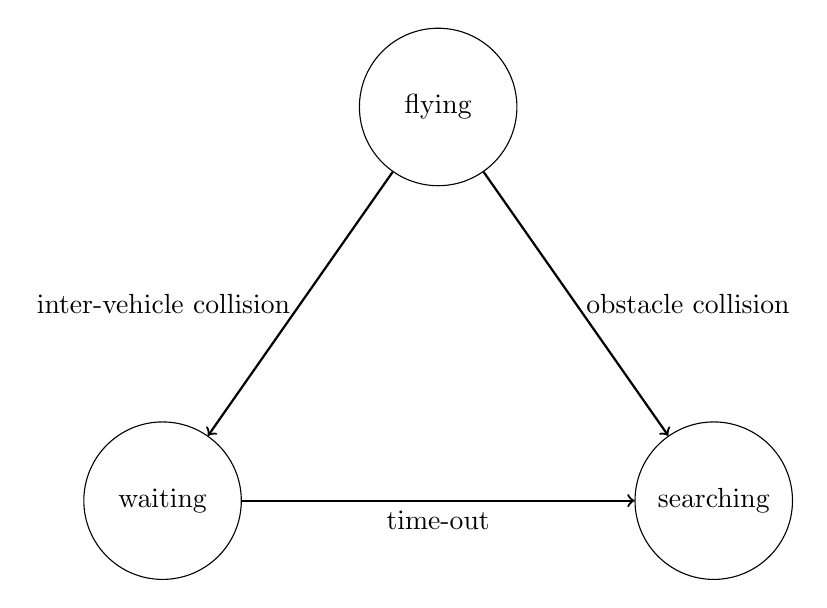
\begin{tikzpicture}
\node[shape=circle, align=center, draw=black, minimum size=2cm] (wa) at (-3.5, 0) {waiting};
\node[shape=circle, align=center, draw=black, minimum size=2cm] (fl) at (0,5) {flying};
\node[shape=circle, align=center, draw=black, minimum size=2cm] (se) at (3.5, 0) {searching};

\path[thick,->] (fl) edge node[left] {inter-vehicle collision} (wa);
\path[thick,->] (fl) edge node[right] {obstacle collision} (se);
\path[thick,->] (wa) edge node[below] {time-out} (se);

\end{tikzpicture}

Most of the time, the state Flying is kept.
Once the set of trajectory nodes are calculated and returned from the algorithm, the UAV follows the nodes and simultaneously predicted a new trajectory. The loop will be continued until another state is switched or the goal point is reached. When there are no available trajectories, and the value of the flag is also equal to True, it can be known that the path is blocked by its teammates instead of obstacles. In this case, the state will be automatically switched to Waiting, where UAVs are required to stop and re-plan the path. Waiting is often seen when avoiding obstacles and formation merging, significantly when the orientation changes quickly. Thus, the later UAVs should give in until the former UAVs pass. However, a deadlock may occur when most UAVs congest in an environment such as a blind alley. To solve such a problem, a time constant Clock is used to prevent a UAV wait overtime. If Clock
exceeds Wait, the state Searching will be invoked.
\[
    waiting()= 
\begin{cases}
    \text{stop and re-plan},& \text{if } clock<t_{wait}\\
    \text{switch to } searching, & \text{otherwise}
\end{cases}
\]

$searching$ is also be used when a UAV has no trajectories found due to the obstacle collision. The UAV stops and rotates its orientation to plan other possible trajectories. In this paper, the orientation is clockwise rotated with a predefined angular velocity $\omega_{search}$. The equation is shown as follows:

\begin{equation}
\begin{aligned}
& \theta_{i}(t) = \theta_{i}(t_{0}) + t \cdot \omega_{search}
\end{aligned}
\end{equation}

In our proposed algorithm, the overall time complexity depends on the time window [$t_{0}$, $t_{T}$]. The big-O notation can be denoted as $O((t_{T})^2)$ due to the changes by $v$ and $\omega$. More specifically, other variables such as velocity acceleration $a$, angular acceleration $\Delta\omega$, and the resolution used in the for-loop in the algorithm also affect the time performance.




